\subsection{Computer program}

I implemented the adaptive \gls{SMC} algorithm for \gls{ABC} developed by
\textcite{del2012adaptive}. The program was written in the
\software{C} programming language. The \software{igraph}
library~\autocite{csardi2006igraph} was used to generate and store contact
networks and phylogenies. Judy arrays~\autocite{baskins2004judy} were used for
hash tables and dynamic programming arrays. The
\gls{GSL}~\autocite{gough2009gnu} was used to generate random draws from
probability distributions, and to perform the bisection step in the
\gls{ABC}-\gls{SMC} algorithm.

For ease of exposition, we simplifiy the notation of \textcite{del2012adaptive}
by dropping the subscripts on the variables which indicate the current
iteration number. Instead, we will add a prime $'$ to indicate a value which
will be used in the next iteration (this should become clear later on). 

In the algorithm, we keep track of a population of $n$ sets of model
parameters, called \defn{particles}, denoted $\set{X_i}_{i=1}^{n}$. For the
\gls{BA} model, the particles would be 4-tuples (\gls{N}, \gls{I}, \gls{m},
\gls{alpha}). Each particle $X_i$ is associated with a set of \gls{M} simulated
datasets, denoted $\set{X_{i,j}}_{j=1}^M$, and a weight $W_i$. 

The particles are initially drawn from the prior distribution.

Let $d$ be a
distance measure on data sets, so that $d(x, y)$ is smaller the more similar
$x$ and $y$ are to each other. Let $\varepsilon$ be the tolerance level which
indicates whether a data set is ``close'' to the observed data. That is, if
$d(x, y) < \varepsilon$, we will say that $x$ and $y$ are close, otherwise they
are distant.

\subsubsection*{Epidemic simulation}
\label{subsubsec:nettree}

I implemented a Gillespie simulation algorithm~\autocite{gillespie1976general}
for simulating epidemics, and the corresponding transmission trees, over static
contact networks. This method has been independently implemented and applied by
several authors~\autocite[\textit{e.g.}][]{o2010contact, robinson2013dynamics,
leventhal2012inferring, groendyke2011bayesian}.
\textcite{groendyke2011bayesian} published their implementation as an
\software{R} package, but since the \gls{SMC} algorithm is quite
computationally intensive, we chose to implement our own version in
\software{C}.

Let $G = (V, E)$ be a directed contact network. The individual nodes and edges
of $G$ follow the dynamics of the \gls{SIR}
model~\autocite{kermack1927contribution}. Each directed edge $e = (u, v)$ in
the network is associated with a transmission rate $\beta_e$, which indicates
that, once $u$ becomes infected, the waiting time until $u$ infects $v$ is
distributed as $\Exponential(\beta_e)$. Note that $v$ may become infected
before this time has elapsed, if $v$ has other incoming edges. $v$ also has a
removal rate $\gamma_v$, so that the waiting time until removal of $v$ from the
population is $\Exponential(\gamma_v)$. Removal may correspond to death or
recovery with immunity, or a combination of both, but in our implementation
recovered nodes never re-enter the susceptible population. We define a
\defn{discordant edge} as an edge $(u, v)$ where $u$ is infected and $v$
has never been infected.

To describe the algorithm, we introduce some notation and variables. Let
$\inc(v)$ be the set of incoming edges to $v$, and $\out(v)$ be the set of
outgoing edges from $v$. Let $I$ be the set of infected nodes in the network,
$R$ be the set of removed nodes, and $S$ be the remaining susceptible nodes,
and $D$ be the set of discordant edges in the network. Let $\beta$ be the total
transmission rate over all discordant edges, and $\gamma$ be the total removal
rate of all infected nodes,
\[
  \beta = \sum_{e \in D} \beta_e, \quad
  \gamma = \sum_{v \in I} \gamma_v.
\]
The variables $S$, $I$, $R$, $D$, $\beta$, and $\gamma$ are all updated as the
simulation progresses. When a node $v$ becomes infected, it is deleted from $S$
and added to $I$, any formerly discordant edges in $\in(v)$ are deleted from
$D$, and edges in $\out(v)$ to nodes in $S$ are added to $D$. If $v$ is later
removed, it is deleted from $I$ and added to $R$, and any discordant edges in
$\out(v)$ are deleted from $D$. In both cases, the variables $\beta$ and
$\gamma$ are updated to reflect the changes. Since these updates are
straightforward, we do not write them explicitly in the algorithm.

\newcommand{\tip}{\mathrm{tip}}

The Gillespie simulation algorithm is given as Algorithm~\ref{alg:nettree}. The
transmission tree $T$ is simulated along with the epidemic. We keep a map
called $\tip$, which maps infected nodes in $I$ to the tips of $T$. The
simulation continues until either there are no discordant edges left in the
network, or we reach a user-defined cutoff of time ($t_{\max}$) or number of
infections ($I_{\max}$). We use the notation $\Uniform(0, 1)$ to indicate a
number drawn from a uniform distribution on $(0, 1)$, and likewise for
$\Exponential(\lambda)$. The combined number of internal nodes and tips in $T$
is denoted $|T|$.

\begin{algorithm}
  \label{alg:nettree}
  \caption{Simulation of an epidemic and transmission tree over a contact network}
  \begin{algorithmic}
    \State infect a node $v$ at random, updating $S$, $I$, $D$, $\beta$ and $\gamma$
    \State $T \gets$ a single node with label $1$
    \State $\tip[v] \gets 1$
    \State $t \gets 0$
    \While{$D \neq \emptyset$ and $|I| + |R| < I_{\max}$ and $t < t_{\max}$}
      \State $s \gets \min(t_{\max} - t, \Exponential(\beta + \gamma))$
      \For{$v \in \tip$}
        \State{extend the branch length of $\tip[v]$ by $s$}
      \EndFor
      \State $t \gets t + s$
      \If{$t < t_{\max}$}
        \If{$\Uniform(0, \beta + \gamma) < \beta$}
          \State choose an edge $e = (u, v)$ from $D$ with probability $\beta_e / \beta$
                 and infect $v$
          \State add tips with labels $(|T|+1)$ and $(|T|+2)$ to $T$
          \Comment $|T|$ increased by 2
          \State connect the new nodes to $\tip[v]$ in $T$, with branch lengths $0$
          \State $\tip[v] \gets |T|-1$
          \State $\tip[u] \gets |T|$
        \Else
          \State choose a node $v$ from $I$ with probability $\gamma_v / \gamma$
                 and remove $v$
          \State delete $v$ from $\tip$
        \EndIf
        \State update $S$, $I$, $R$, $D$, $\beta$, and $\gamma$
      \EndIf
    \EndWhile
  \end{algorithmic}
\end{algorithm}

\subsubsection{Phylogenetic kernel and normalized lineages-through-time}

The tree kernel developed in~\autocite{poon2013mapping} provides a
comprehensive similarity score between two phylogenetic trees. The kernel
computes the dot-product of two feature vectors, corresponding to the two
trees, in the infinite-dimensional feature space of all possible subset trees
with branch lengths. I implemented the fast algorithm developed
in~\autocite{moschitti2006making}, which first enumerates all pairs of subtrees
with the same number of leaf children, and then computes the kernel by dynamic
programming.

In addition, we implemented a modified version of the normalized
lineages-through-time statistic developed in~\autocite{janzen2015approximate},
which uses piecewise linear functions instead of step functions for the
lineages-through-time plots. This modification is to address a potential
inconsistency for trees of different sizes, illustrated in
Figure~\ref{fig:nltt}.

\begin{figure}[ht]
  \centering
  \caption[Comparison of original and modified normalised lineages-through-time]
    {Comparison of original formulation of normalized lineages-through-time,
     developed in~\autocite{janzen2015approximate}, with our modified version
     using linear interpolation. Here, the red and blue trees both have
     uniformly spaced branching times. Using step functions (left), the nLTT
     of the two trees is non-zero due to the differing numbers of internal
     branches. Using linear interpolation, the nLTT is zero (right). The lines
     on the right graph have been offset for visibility.}
  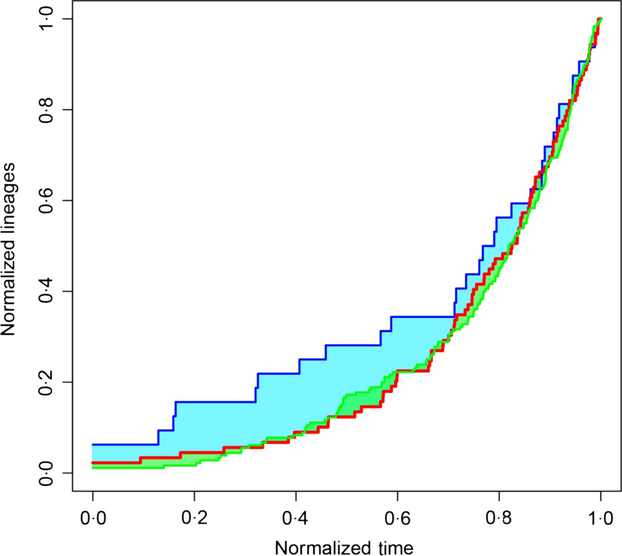
\includegraphics{nltt.pdf}
  \label{fig:nltt}
\end{figure}


% begin by sampling from the prior and setting all weights to equal

Next, we calculate the next tolerance $\varepsilon^*$. Before we explain how
this is done, we first need to define how we adjust the weights on the
particles. As explained above (see subsection~\ref{subsubsec:abcalg}), the idea
of sequential Monte-Carlo is to begin with the prior distribution $\pi$,
progress smoothly through a series of intermediate distributions $\pi_1,
\ldots, \pi_{n-1}$, and eventually arrive at the target posterior distribution
$\pi_n$. In the $k$th iteration, the distribution $\pi_k$ is approximated by
the particles and their weights. 

In contrast to most existing sequential Monte-Carlo methods, this
algorithm does not require the user to specify a sequence of decreasing
tolerances to approach the target posterior distribution. Rather, the
tolerances are computed adaptively at each step, starting from infinity at the
first iteration. 

The algorithm may be stopped when the tolerance reaches a
user-defined final value, or when the rate of acceptance of the
Metropolis-Hastings kernel reaches a user-defined threshold. Following a
heuristic applied by the authors~\autocite{del2012adaptive}, we used the latter
stopping criterion, accepting the SMC approximation to the posterior when the
\gls{MCMC} acceptance rate dropped below 1.5\%.

\subsection{Simulation experiments}

\subsubsection{Identification of separable parameters in kernel space}
\label{subsubsec:kernel}

Recall that our approximate Bayesian computation approach to fitting contact
network models involves simulating transmission trees under a wide variety of
parameter values, and then comparing these simulated trees to the true
transmission tree. Values which produce trees similar to the observed
transmission tree are distinguished as more likely than values which produce
trees very different from the truth. In order for this type of analysis to
succeed, it is critical that different parameter values produce different
looking trees. Otherwise, if many different values produce trees which are too
similar to each other, it will be impossible to distinguish which value is most
consistent with the real tree. Just as importantly, trees simulated with
similar parameter values must be similar to each other. In mathematical terms,
we require the trees simulated from distinct parameter values to be
\defn{separable} in tree space. The concept of separability is illustrated in
Figure~\ref{fig:separable}.

\begin{figure}[ht]
  \centering
  \includegraphics{separable.pdf}
  \caption[Separable versus non-separable pararameters in kernel space]{
    Separable versus non-separable parameters in kernel space. Trees have been
    simulated under three sets of parameters, represented as blue, red, and
    green. An observed tree is shown in black. Trees are layed out such that
    the distance between two trees corresponds to their similarity. In panel A,
    trees from the same parameter set are similar to each other, but different
    from other trees. The true tree is most consistent with the red parameters.
    In panels B and C, trees from the same parameter set are not similar to
    each other (B), or trees from different parameter sets are similar to each
    other (C). It's difficult to say which parameters the true tree is most
    consistent with.
  }
  \label{fig:separable}
\end{figure}

Before undertaking a complete ABC analysis, I analysed the parameters of the
\gls{BA} network model to to determine whether they could be separated in tree
kernel space. A graphical schematic of the analysis undertaken here is given in
Figure~\ref{fig:kernelexpt}.

\begin{figure}[ht]
  \centering
  \label{fig:kernelexpt}
  \includegraphics{kernel-expt.pdf}
  \caption[Schematic of first set of simulation experiments]{
    Schematic of first set of simulation experiments to determine separable
    parameters in kernel space, along with optimal tree kernel meta-parameters.
  }
\end{figure}

The method of testing for separability was described previously
in~\autocite{poon2015phylodynamic}. As a concrete example, consider the
attachment power parameter \gls{alpha}. This parameter describes the strength
of attraction to highly connected nodes and is bounded below by zero indicating
no extra attraction. By qualitative observation, I determined that a power of
2.0, which produced networks with very few ``hub'' nodes with extremely high
degree, was a suitable upper bound (see Figure~\ref{fig:alphabds}). Therefore,
I chose to test the values 0.5, 1.0, and 1.5 for separability. The other
parameters were fixed: the number of nodes in the network was 5000, and the
mean degree of each node in the network was four. As discussed in
subsection~\ref{subsubsec:generative}, this is the smallest mean degree value
for preferential attachment networks which produces networks which are more
than trees. 

\begin{figure}[ht]
  \centering
  \label{fig:alphabds}
  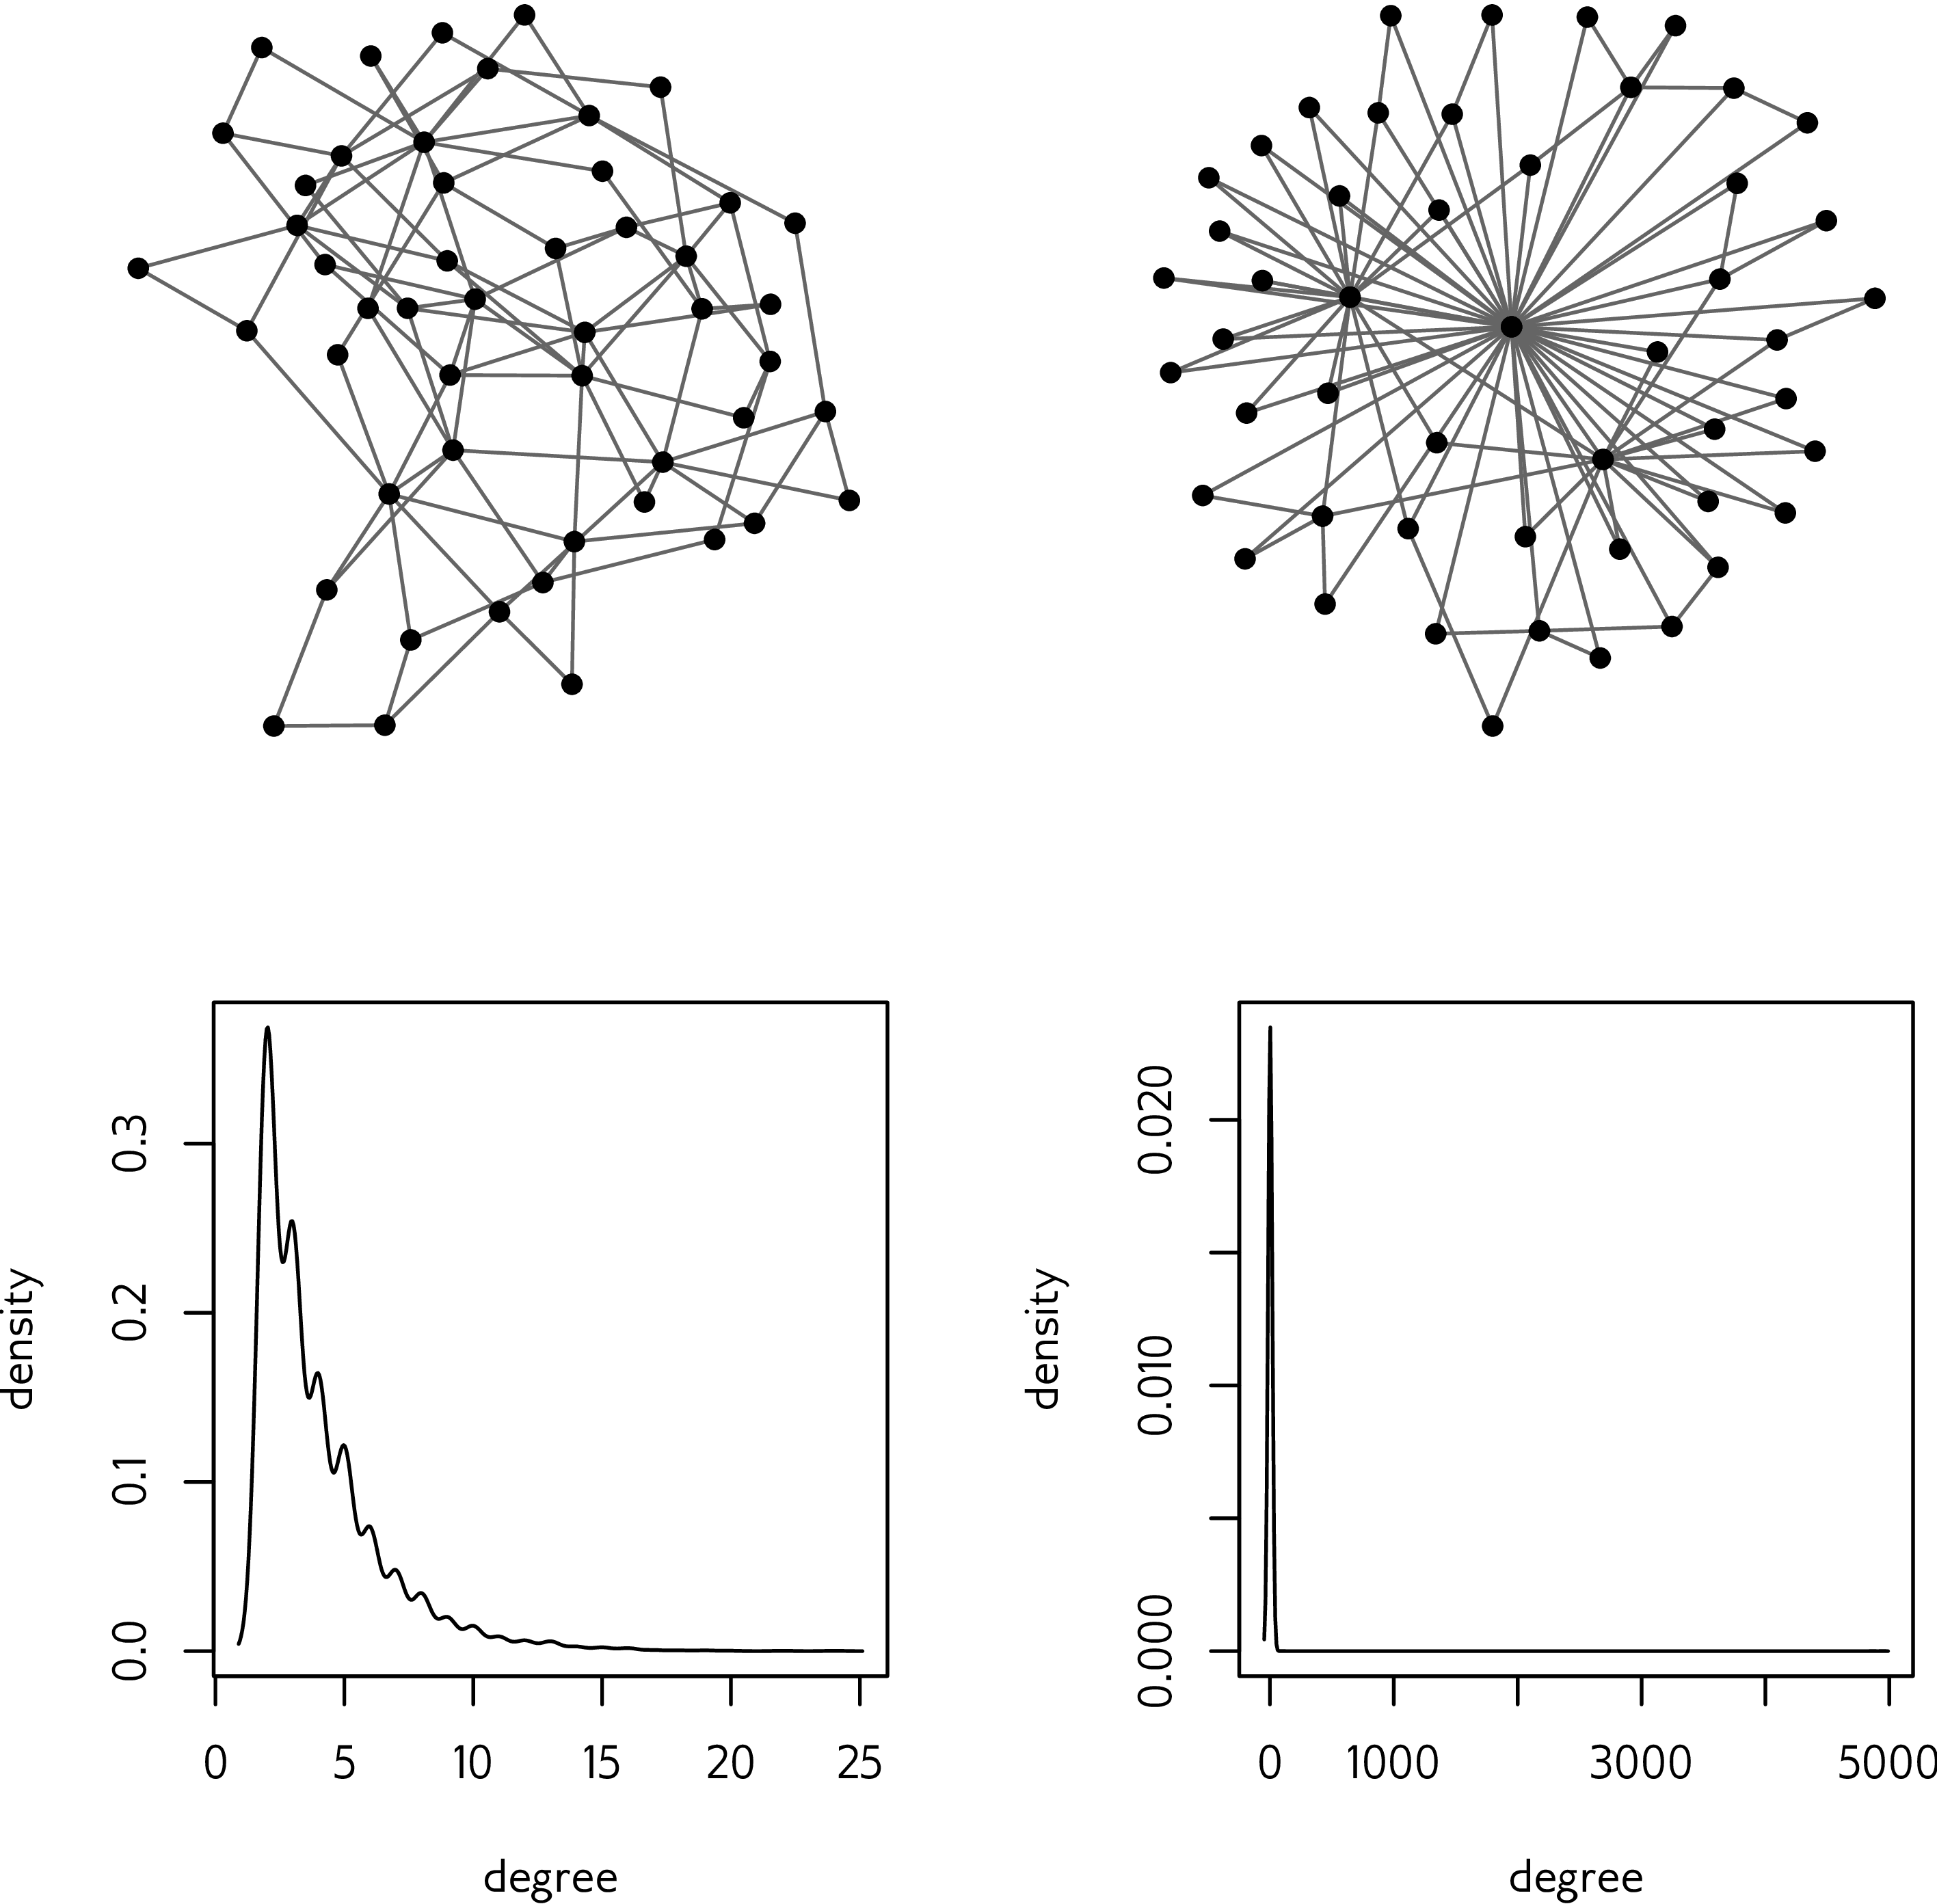
\includegraphics{alpha-bounds.pdf}
  \caption[Upper and lower bounds on preferential attachment power]{
    Qualitative justification for choice of zero and two as lower and upper
    bounds on preferential attachment power $\alpha$. (A) Preferential
    attachment network on 50 nodes with $\alpha = 0$, the lower bound enforced
    by the model. (B) Preferential attachment network on 50 nodes with $\alpha
    = 2$, where a few nodes have very high degree but the majority have very
    low degree. (C) Density plot of node degrees in a 5000-node network with
    $\alpha = 0$. The maximum degree of a node in this network was 24. (D)
    Density plot of node degrees in a 5000-node network with $\alpha = 2$. The
    maximum degree of a node in this network was 4942. 
  }
\end{figure}

For each of the values of $\alpha$, I generated 100 networks, each with 5000
nodes. An epidemic was simulated over each network (see
\cref{subsubsec:nettree}) until 1000 nodes were infected, and 500 of those
infected nodes were sampled to form a transmission tree. This resulted in 300
total simulated transmission trees - 100 for each of the three values of
$\alpha$. The data generation steps are shown on the left side of
Figure~\ref{fig:kernelexpt}. Next, I computed the tree
kernel~\autocite{poon2013mapping} (see subsection~\ref{subsubsec:treeshape})
for each pair of trees. These values were placed into a 300 $\times$ 300 kernel
matrix, where the value at the $(i, j)$th position was the tree kernel of the
$i$th and $j$th trees. 

The tree kernel provides a pairwise similarity score between two trees. The
higher the kernel score, the more similar the trees are to each other.
Therefore, to have separability, we need trees simulated with the same value of
$\alpha$ to have high kernel scores with each other, but low kernel scores with
trees from different $\alpha$ values. We can visually check whether or not this
is true by laying out the trees as points on a graph, in such a way that trees
with high scores are close to each other, but trees with low scores are far
apart. This is accomplished by performing a kernel principal components
analysis (kPCA)~\autocite{scholkopf1998nonlinear} on the kernel matrix.
Briefly, ordinary principal components analysis (PCA) finds a lower dimensional
representation of points in a high dimensional space which preserves as much of
the variation in the data as possible. kPCA performs the same task, but using
the dot products of each pair of points as input, instead of the data points
themselves. A two-dimensional kPCA projection of the simulated trees is shown
in Figure~\ref{fig:pakpca}. The scenario just described - 500 samples from 1000
infected nodes - is the central panel. To ensure that the method could be used
in a variety of contexts, the same analysis was performed with 500 and 2000
infected nodes, as well as 100 and 1000 sampled tips. 

The next step was to quantify how well trees simulated with different $\alpha$
values could be distinguished from each other. As described
previously~\autocite{poon2015phylodynamic}, this was done by assessing the
accuracy of a support vector machine regression
(SVR)~\autocite{smola1997support}. Briefly, an SVR operates by finding a
hyperplane (in two dimensions, a line) such that the deviation of most of the
data points from the line is less than some prescribed threshold. Points
further away than this threshold are ignored in the model. I performed 1000
replicate 2-fold cross-validations of an SVR predicting preferential attachment
power on the simulated trees, using the \software{ksvm} function from
\software{kernlab}~\autocite{karatzoglou2004kernlab}. That is, the SVR was
trained on a random subset of 150 trees, and then used to predict $\alpha$ of
the remaining 150 trees. The predictions were correlated against the true
values of $\alpha$ to obtain an $R^2$, and this procedure was repeated 1000
times with different subsets of trees.

The cross-validation had the dual purpose of providing a means to selecting the
optimal meta-parameters to the tree kernel (see
subsection~\ref{subsubsec:treeshape}) - they are be those which provide the
highest average $R^2$. To this end, the cross-validation was repeated for
several values of $\lambda$ and $\sigma$ as shown in Figure~\ref{fig:kernelexpt}
Each combination was evaluated with and without multiplying the tree kernel by
the normalized lineages-through-time (nLTT) statistic, and was further repeated
for the scenarios with differing numbers of infected and sampled nodes
described above. To ensure that the tree kernel was the most appropriate
similarity measure to use for ABC, we also computed the $R^2$ of $\alpha$
against Sackin's index, a widely used tree balance statistic (see
subsection~\ref{subsubsec:treeshape}), by the same cross-validation procedure.

\subsubsection{Grid search}

The previous set of simulations were intended to investigate which contact
network parameters could and could not be inferred by examining transmission
trees. However, they tell us nothing about the accuracy or precision we might
expect when inferring those parameters numerically. As illustrated in
Figure~\ref{fig:accprec}, the ideal situation is one where we are accurate and
precise, and the worst situation is when we are precise but not accurate.

\begin{figure}[ht]
  \centering
  \includegraphics{acc-prec.pdf}
  \caption{Illustration of accurate vs. precise kernel score estimates}
  \label{fig:accprec}
\end{figure}

Figure~\ref{fig:gridsearch} shows a schematic of this experiment. A number of
representative values, here denoted $k$, were chosen for the parameter of
interest. In the case of preferential attachment power $\alpha$, I chose $k =
8$ testing values, namely $0, 0.25, \ldots, 2.0$. For each of these values, ten
networks on 5000 nodes were generated, an epidemic of 1000 nodes was simulated
over each, and a transmission tree of 500 tips was sampled. The resulting $10
\times k$ simulated transmission trees were referred to as the \defn{testing
trees}. In addition, I chose a further $n \gg k$ training values spanning the
range of the parameter. For $\alpha$, these were $0, 0.01, \ldots, 2.0$.
Fifteen trees were simulated in the same manner for each of these values,
referred to here as \defn{training trees}.

For each of the testing trees, I computed the tree kernel with all of the
training trees. This resulted in 15 kernel scores per training value. The
training value with the highest median kernel score was used as a point
estimate of the testing value. The kernel scores were then normalized to lie in
[0, 1], and an interval was found which contained 95\% of the area under the
curve and was of minimal width. This was used as a 95\% confidence interval for
the parameter.

\begin{figure}[ht]
  \centering
  \includegraphics{gridsearch-expt.pdf}
  \caption{Schematic of grid search simulation experiments.}
  \label{fig:gridsearch}
\end{figure}

\subsubsection{Approximate Bayesian computation}

Our final set of simulation experiments was to test the ABC-SMC algorithm on
simulated data. For each replicate, we generated a network on 5000 nodes,
simulated an epidemic over that network until 1000 nodes were infected, and
sampled either 500 or all 1000 of those nodes to form a transmission tree.
Priors were specified as follows: for the total number of nodes in the network,
$\Uniform(1000, 10000)$; for the number of infected nodes, $\Uniform(500,
2000)$; for the preferential attachment power, $\Uniform(0, 2)$. The mean
degree of nodes in the network was fixed at either 4, 10, or 16. The
algorithm was run with 1000 particles, and was stopped when the \gls{MCMC}
acceptance probability dropped below 1.5\%.

\subsubsection{Characterization of power-law exponent in Barab\'asi-Albert networks}

Most studies of social network or transmission network
parameters~\autocite[e.g.][]{liljeros2001web, jones2003assessment,
schneeberger2004scale, brown2011transmission} report the coefficient
\gls{gamma} of the power law degree distribution. To make our results
comparable to previous work, we used simulated networks to investigate the
relationship between the \gls{BA} model parameters and \gls{gamma}. A network
was simulated for each element of the Cartesian product of these parameters:
\gls{N} = \sett{500, 600, \ldots, 15000}, \gls{m} = \sett{1, 2, \ldots, 8}, and
\gls{alpha} = \sett{0.00, 0.01, \ldots, 2.00}. A power law distribution was
fitted to the degree distribution of each simulated network using the
\software{fit\_power\_law} function in \software{igraph} with the `R.mle'
implementation. We fitted a \gls{GLM} with Gamma-distributed errors and a log
link function to the observed distribution of \gls{gamma} values, with
\gls{alpha}, \gls{m}, \gls{N}, and all possible interaction terms as
predictors.

\subsection{Real data experiments}

We applied kernel-ABC to six published HIV datasets, summarized in
\cref{tab:realdata}.

\begin{table}
  \centering
  \begin{tabular}{ccccc}
  Reference & Sequences ($n$) & Location & Risk group & Gene \\
  \hline
  \textcite{wang2015targeting} & 173 & Beijing, China & MSM & \textit{pol} \\
  \textcite{cuevas2009hiv} & 287 & Basque Country, Spain & mixed & \textit{pol} \\
  \textcite{novitsky2013phylogenetic} & \multirow{2}{*}{180} &
  \multirow{2}{*}{Mochudi, Botswana} & \multirow{2}{*}{HET} &
  \multirow{2}{*}{\textit{env}} \\ \textcite{novitsky2014impact} \\
  \textcite{li2015hiv} & 280 & Shanghai, China & MSM & \textit{pol} \\
  \textcite{niculescu2015recent} & 136 & Romania & IDU & \textit{pol} \\
  unpublished & 399 & British Columbia, Canada & IDU & \textit{pol} \\
  \hline
\end{tabular}

  \caption{Characteristics of published HIV datasets analysed with kernel-ABC.}
  \label{tab:realdata}
\end{table}
